\input preamble.tex
\startEntry{}
Today's lecture will be about frying.
\section{How to fry and egg}
There are lots of different ways to fry an egg, but they all do a similary thing: Heat the egg up so that it cooks in, but in a frying pan. I will now describe how to do this.
\begin{enumerate}
\item Put pan on heat
\item Add fat (oil, butter)
\item Let oil heat up a bit
\item Add egg
\item (Optional) Stir egg violently
\item When egg is no longer liquid, it is cookes
\item Remove egg
\item Take pan off heat
\end{enumerate}
I should probably mention that I have never cooked an egg before.
This is what it shoud look like:
\begin{figure}[h]
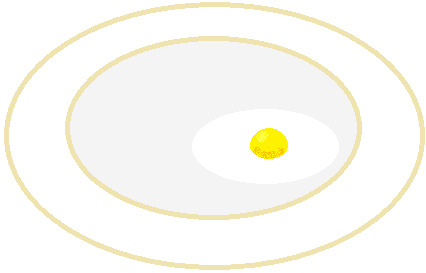
\includegraphics[width=8cm]{Egg_on_plate.png}
\end{figure}


Now isn't that a nice egg?
\finishEntry{}